\section{Introduction}
\label{ref_intro}

Over the course of 3 years, 6 partner universities are developing a \textbf{F}ramework for the \textbf{I}dentification of \textbf{R}are \textbf{E}vents Via \textbf{Ma}chine Learning and IoT \textbf{N}etworks known as the FIREMAN project. According to \cite{fireman-homepage}:
\begin{displayquote}
The project aims to build an architecture with a strong interplay among several research areas, i.e., large-scale data acquisition, big data fusion and big data analytics, towards a highly-integrated cyber-physical system design at all data-processing levels. The overall object of FIREMAN is to design, develop and showcase a novel big-data based framework that encompasses all steps from sensing and data acquisition to statistical analysis and operational decisions, to accurately identify, detect, forecast, and prevent rare events in a pre-determined industrial physical process.
\end{displayquote} 

Although there are many sub-systems and research components of the FIREMAN project, this work will primarily focus on the effective demonstration of the system as a whole. In order to showcase the effectiveness and value of the project, it is essential to demonstrate its feasibility and usability to stake holders and end users. In any scientific work it is always a challenge to convey the information and deliverables to stake holders of various backgrounds and disciplines. This work will propose two methods of accomplishing this goal: digital simulation demonstrations and practical low-cost physical demonstrations. These two approaches will demonstrate the effectiveness and viability of the FIREMAN system and which will demonstrate a value proposition to the CHIST-ERA program that funded the project and other stake holders. 

\subsection{Project Structure}

FIREMAN is multidisciplinary cooperation between 6 universities in 4 different countries as stated in section \ref{ref_intro}. Lappeenranta University of Technology (LUT) serves as the project coordinator and is involved in all aspects of the project. The project is partitioned into seven overall Work Packages (WPs) that define overall sub-tasks to meet the general project objective. The interconnection and overview of the individual WPs is shown in figure \ref{fig:wp-diagram}.

\begin{figure}[H]
    \centering
    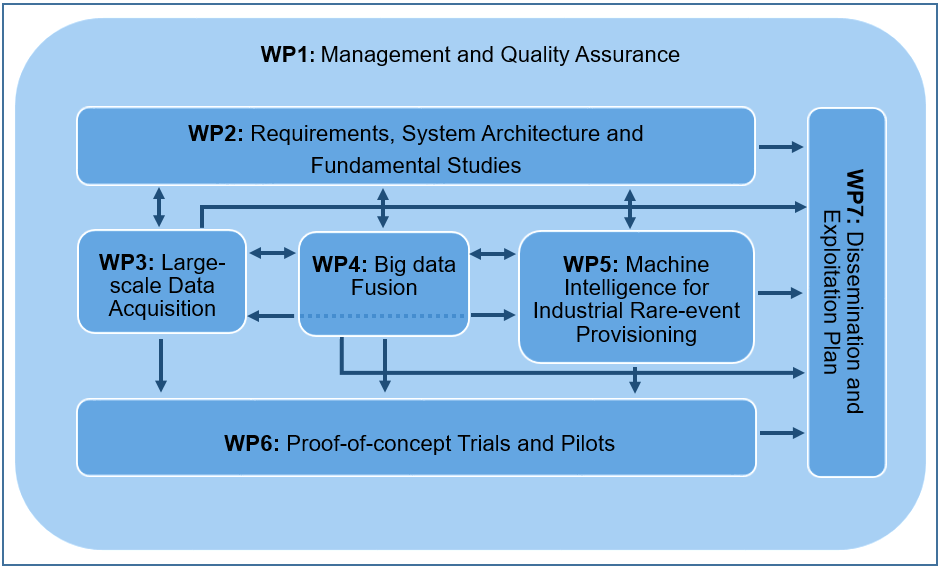
\includegraphics[width=0.8\textwidth]{Images/FIREMAN_pert_diagram.png}
    \caption{FIREMAN WP Diagram}
    \label{fig:wp-diagram}
\end{figure}

According to \cite{fireman-about} WP3, WP4, and WP5 will accomplish the following:
\begin{displayquote}
WP3 will focus on the collection and acquisition of heterogeneous data captured by many sensors embedded into various devices and machines in the physical world. This WP will further investigate secure ultra-reliable data transfer and communication while network architecture aspects will be also considered. Aggregated sensor data combined with data fusion, mining, and interpretation will enable efficient control and awareness of the physical processes. This is the objective of WP4 where advanced machine learning techniques will be developed to convert the pre-processed raw sensor data to useful information and allow for preliminary analysis and short-term operational decisions. WP5 will focus on employing big data analytics and artificial intelligence for statistical analysis and knowledge processing to detect/predict/prevent rare events and propose techniques for actuator response.
\end{displayquote}

This work will focus on WP6 with the goal of demonstrating with real and virtual demonstrations a cohesive system incorporating all the advances made in WP3-WP5.  

\subsection{Motivation}

Researchers, Engineers, and Industry Professionals can utilize this work to improve decision making and accuracy in a wide variety of systems. There is currently a gap in the field between the cutting edge theoretical research and applying it to relevant problems and domains. In order to bridge this gap, the researchers must first understand the relevant research, in this case in outlier detection, and then experiment with implementations to determine where it is best suited for practical applications. This will improve the sharing of knowledge and allow multiple domains to benefit from breakthroughs in specific areas. This yields many benefits including, power savings from improved industrial control of electrical process, improved profit from better control over electrical production output, and improved efficiency and accuracy in decision making processes.

The problem is of high importance because current industrial control processes cannot detect or handle anomalies. A PID controller cannot determine or compensate for sensor failure or adversarial data. Additionally, applying machine learning in the domain of power systems and industrial processes is a novel idea and rapidly gaining interest. In this domain, it is critical to provide explainability into the machine learning algorithms to confirm they do not react unexpectedly to certain adversarial inputs. If they act erratically it could lead to large negative safety and financial implications in a way that it would not in other fields.


\subsection{Research Problem}

There are many existing techniques for outlier detection in a variety of disciplines from machine learning for batch data to conventional statistical approaches. These techniques are usually siloed and are not considered as compatible together. This research proposes to break that barrier and use the best technique for the problem.

A relatively new area of research is applying machine learning techniques to industrial systems with data streams. Streaming or “online” machine learning algorithms are unable to look at the data multiple times and must act on and update the model as new datapoints arrive. There is a research gap in implementing and testing these algorithms against existing methods for stream anomaly detection (ex. Half-Space Trees) in popular libraries as many of them are 2-3 years behind current breakthroughs.

These techniques for anomaly detection and machine learning in general are also very new in the field of power electronics and using a machine learning pipeline to improve over an existing PI controlled system is quite novel. Many machine learning algorithms rely on a black box that will output answers provided inputs. This is not suitable for system critical applications like power systems where it is essential to understand why an algorithm is making a specific decision. The algorithms explainability will be analyzed and methods will be proposed so that it is precisely clear why the algorithm is making certain decisions based on input data. This will also be used to analyze what happens when adversarial data enters the system and analyzed from a cyber-security standpoint to design a controller that can defend against potential threats from adversarial inputs.

The resultant algorithm will provide an explainable model that can be used to control industrial processes. The goal is to detect adversarial or anomalous data, and take preventative measures to mitigate its impact.


\subsection{Research Questions}
With this work the researchers hope to answer the following questions:
\begin{itemize}[leftmargin=1cm]
    \item Why do machine learning techniques lack general adoption in the power systems domain
    \item How can machine learning techniques be used to enable increased explainability, performance, and security in system critical applications?
    \item What existing machine learning libraries are available for streaming time series analysis and how can their performance be improved?
    \item Why is there a lack of standardization in modern datasets to test and benchmark anomaly detection machine learning algorithms?
    \item How can different anomaly detection techniques (conventional statistics, deep learning, etc.) be combined (ensembled) to increase overall prediction capability and accuracy?
\end{itemize}

\subsection{FIREMAN Research Team}

\textbf{Alexander Beattie (LUT)} is a Fulbright-LUT University Graduate Award Scholar studying a Master’s of Mechatronic System Design. He has experience working on interdisciplinary engineering projects in cyber-physical systems, electronics, and computer science domains. His thesis work is focused on machine learning techniques for rare event detection and anomaly detection in streaming data. He is also conducting research in industrial cyber-physical systems as part of FIREMAN project and in fundamental limits of packetized energy management for households as part of EnergyNet; both under the supervision of Assoc. Prof. Nardelli. He also has working experience in software development. 

\textbf{Pedro H. J. Nardelli (LUT)} earned his B.S. and M.Sc. degrees in electrical engineering from the State University of Campinas, Brazil, in 2006 and 2008, respectively. In 2013, he received his doctoral degree from the University of Oulu, Finland, and the State University of Campinas following a dual degree agreement. He is currently an associate professor (tenure track) in the Internet of Things (IoT) in energy systems at the Lappeenranta-Lahti University of Technology (LUT University), Lappeenranta, 53850, Finland, and holds the position of Academy of Finland Research Fellow with the project Building the Energy Internet as a Large-Scale IoT-Based Cyberphysical System, which manages the energy inventory of distribution grids as discretized packets via machine-type communications (EnergyNet). He leads the Cyber-Physical Systems Group at LUT University and is project coordinator of the CHIST-ERA European consortium Framework for the Identification of Rare Events via Machine Learning and IoT Networks. He is also a docent at the University of Oulu in communications strategies and information processing in energy systems. His research focuses on wireless communications, particularly applied in industrial automation and energy systems. He received a best paper award of the IEEE Power \& Energy Society Innovative Smart Grid Technologies Latin America 2019 in the track “Big Data and Internet of Things.”

\textbf{Pavol Mulinka (CTTC)} is a Ph.D. candidate at the Faculty of Electrical Engineering, Czech Technical University in Prague, Telecommunications department. He received his M. Eng. at Faculty of Electrical Engineering and Information Technology, Slovak University of Technology in Bratislava, Telecommunications department. During the years 2018-2019, he held visiting researcher positions at AIT Vienna, O2 Telefonica Barcelona, and NII Tokyo. During his Ph.D. studies from 2013 to 2020, he contributed to academia(CTU Prague) and industry (Cisco) funded projects as Principal/Co-investigator. Starting from his Bc. studies at STU in Bratislava (2007), he worked as a full-time network engineer and consultant until 2018. After finishing his Ph.D. thesis, he started contributing to the FIREMAN project as a data science volunteer in February of 2020. He became a full-time research team member in November of 2020. He is also an active data science volunteer at Wikimedia foundation, currently working on integrating the CJK tokenization features into the Wikimedia Python eco-system.

\textbf{Subham Sahoo (Aalborg Universitet)} is currently working with the Department of Energy Technology, Aalborg University, Denmark. His research interests include control and stability of microgrids, renewable energy integration, cyber-physical power electronic systems and cyber security in power electronic systems.,Dr. Sahoo is a recipient of the Indian National Academy of Engineering (INAE) Innovative Students Project Award for his Ph.D. thesis across all the institutes in India in 2019. He has also won the IRD Student Start-Up Award in 2017 to incorporate a company named Silov Solutions Pvt. Ltd. commercialized and based on his contributions during his doctoral studies. He was also one of the outstanding reviewers for the IEEE Transactions on Smart Grid in 2020. He currently serves as a Secretary of IEEE Young Professionals Affinity Group, Denmark, and Joint IAS/IES/PELS in Denmark section.

\textbf{Daniel Gutierrez-Rojas (LUT)} received the B.Sc. degree in Electrical Engineering from University of Antioquia, Colombia in 2016 and the M.Sc. degree in Protection of Power Systems University of São
Paulo, Brazil, in 2017. From 2017 to 2019, he worked as security of operation and fault analyst for Colombia’s National electrical operator. He is currently working toward the Ph.D. degree at the School of Energy Systems at LUT University, Finland. His research interests include predictive maintenance, power systems, microgrids, mobile communication systems and electrical protection systems.


\textbf{Ioannis Christou (ACG)} is a Senior Research Data Scientist at INTRASOFT Intl, Lux. and a part-time faculty member at ACG. He has over 25 years academic and industrial experience in the IT sector. Dr. Christou’s current teaching at ACG involves Databases at the undergraduate level, and Applied Machine Learning \& Advanced Machine Learning at the graduate level. He has taught as Full Professor at AIT, Greece, and as Adjunct Professor at Carnegie-Mellon University, USA, Aalborg University, Denmark, Democritus University of Thrace and the University of Patras, Greece. Dr. Christou’s research interests include Scalable Data Mining, Parallel and Distributed Computing and Optimization and Computational Intelligence. He has published over 90 papers and a book. He is Academic Editor of the journal Mathematical Problems in Engineering.

\textbf{Charalampos Kalalas (CTTC)} received the Ph.D. (Cum Laude) degree in Signal Theory and Communications from the Universitat Politècnica de Catalunya (UPC) in 2018. He holds an Electrical and Computer Engineering degree (2011) and an M.Sc. degree in Wireless Systems (2014) from the National Technical University of Athens (NTUA) and the Royal Institute of Technology (KTH), respectively. In 2014, he was the recipient of the ISSLS-2000 award by KTH-ICT School for his Master thesis. During the years 2013-2017, he held visiting researcher positions both in the Industry (Ericsson Eurolab and ABB Corporate Research) and Academia (KTH and Aalborg University).

\subsection{FIREMAN Research Consortium}
The FIREMAN consortium comprises 6 partners located in 4 European countries, consisting of 3 universities, 2 research centers and 1 automotive company. The composition of FIREMAN consortium has been carefully selected in order to include all necessary competences and resources to carry out research at the intersection of wireless IoT connectivity and machine learning towards end-to-end predictive and automated industrial systems. Complementary skills among the partners have been chosen to span the sufficient space of cross-disciplinary expertise required by FIREMAN to successfully carry out the project objectives and create impact.

\textbf{Lappeenranta University of Technology (LUT)} is the FIREMAN project coordinator. LUT is involved in all WPs. Besides management and dissemination, LUT is involved in the system architecture, physical system modelling, data acquisition and sampling strategies, data aggregation transmission and compression, visualization of rare events, as well as in the integration tests in its industrial settings (e.g., bearing condition monitoring, pump, blower and compressor faults and wind turbine maintenance).

\textbf{Athens Information Technology (AIT)} leads the FIREMAN technical management activities. Prof. Papadias is the Technical Coordinator of the project. AIT leads WP5, and in particular Task 5.1 where most of the research on developing novel beyond state-of-the-art machine learning and data mining methods for detecting rare events that imply the need for predictive maintenance in smart industry will be carried out. AIT leads also Task 2.3 in WP2, with a focus on deriving theoretical properties on the processes generating events for the algorithms of Task 5.1 to be able to reliably detect them.

\textbf{Centre Tecnològic de Telecomunicacions de Catalunya (CTTC)} is the WP3 leader in FIREMAN. CTTC coordinates the research activities of WP3 as well as contributes to both Task 3.1 and Task 3.3 with data modelling and data transmission protocols, respectively. In addition, CTTC contributes to WP2 by defining scenarios and KPIs, to WP4 by designing data fusion algorithms, and to WP6 by working closely with SEAT in the pilot activities. CTTC actively contributes to the project’s dissemination activities. 

\textbf{Trinity College Dublin (TCD)} leads WP4 and Task 4.2, focusing on developing distributed filtering approaches for data reduction and machine learning techniques for dimensionality reduction. TCD leads Task 5.3, focusing on maintenance schedule optimization. TCD is part of Task 7.1 leveraging CONNECT’s powerful networks, industrial partnerships and additional multipliers channels to raise the visibility of FIREMAN.

\textbf{University of Oulu} and, in particular the Centre for Wireless Communications (CWC), leads the activities of WP6 as well as Task 4.1, and contributes to WP2-WP7 of FIREMAN. UOULU is involved in the physical system modelling, data gathering (event based and clustering), in developing stochastic data aggregation and compression and coordinates the activities for deployment in industrial settings.

\textbf{SEAT} will provide a key manufacturing challenge for which innovative solutions based on Internet of Things and Artificial Intelligence will be required. The challenge will be related to predictive maintenance of production machines (such as, painting robots, presses, etc.) and will consist in how to automatically detect and predict when a given machine will stop working. SEAT will define the requirements of the predictive maintenance use case and will provide production data so that other partners of the project can develop the best solutions. Then, SEAT will integrate, test, and validate the proposed solutions in its facilities, in controlled environments. In addition, SEAT will contribute to the dissemination of results by posting updates about FIREMAN in social networks and giving talks and presentations about the project in top-level industrial congresses, fairs, and industrial events (such as, Internet of Manufacturing, Advanced Factories, IoT Solutions World Congress, Mobile World Congress, etc.), in Volkswagen Group guild meetings, and in universities and research centers to strengthen the importance of collaboration between academia and industry. All in all, SEAT will contribute in all technical WPs as well as in the dissemination activities by defining the plan for the exploitation of FIREMAN results in WP7.
